\begin{definicja}
  Niech \(\to\) będzie relacją binarną w zbiorze \(A\). 
\begin{enumerate}
  \setlength\itemsep{0em}
  \item[(CR) ] Powiemy, że \(\to\) ma \emph{własność Churcha-Rossera}, jeśli
               dla dowolnych \(a,\,b,\,c\in A\) takich, że
               \(a\to^{*}b\) oraz \(a\to^{*} c\) istnieje \(d\in A\)
               takie, że \(b\to^{*} d\) i \(c\to^{*} d\).\label{def:cr_property_untyped}
               Innymi słowy, przemienny jest diagram:
               \[ \begin{tikzcd}
               a \arrow{r}{*} \arrow[swap]{d}{*} & b \arrow{d}{*} \\%
               c \arrow{r}{*}& d
               \end{tikzcd}
               \] 

  \item[(WCR)] Powiemy, że \(\to\) ma \emph{słabą własność 
               Churcha-Rossera}, jeśli dla dowolnych \(a,\,b,\,c\in A\)
               takich, że \(a\to b\) oraz \(a\to c\) istnieje \(d\in A\) 
               takie, że \(b\to^{*} d\) i \(c\to^{*} d\).\label{def:wcr_property_untyped}
               Innymi słowy, przemienny jest diagram:
               \[ \begin{tikzcd}
               a \arrow{r}{} \arrow[swap]{d}{} & b \arrow{d}{*} \\%
               c \arrow{r}{*}& d
               \end{tikzcd}
               \] 

\end{enumerate}
  Widzimy, że własność CR pociąga za sobą własność WCR. Odwrotna zależność nie zachodzi (patrz Rysunek \ref{fig:wcrnotcr}).
\end{definicja}

\begin{figure}[!h]
  \centering
  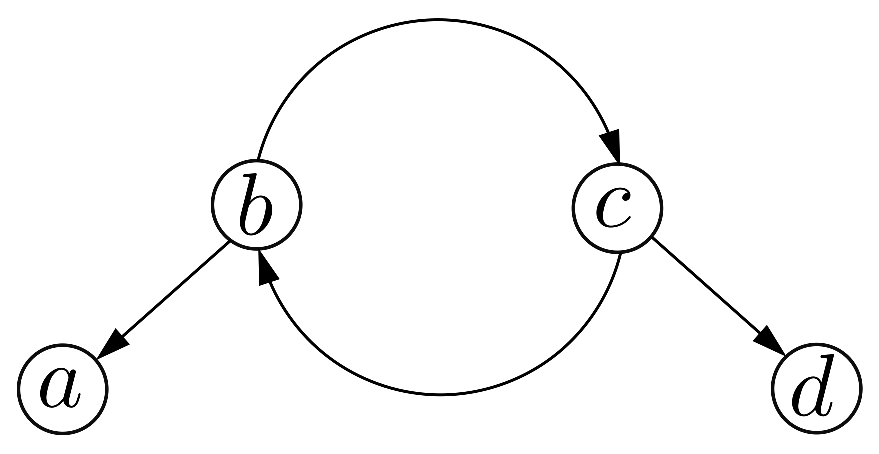
\includegraphics[width=0.32\linewidth]{../wcrnotcr_example}
  \caption{Rozważmy graf skierowany, w którym krawędzie odpowiadają relacji \(\to\) w zbiorze \(\{a,b,c,d\}\). Widzimy, że relacja \(\to\) ma własnosność WCR, ale nie ma własności CR.}\label{fig:wcrnotcr}
\end{figure}

\begin{definicja}(Postać normalna)
  Powiemy, że \(x\in A\) jest \emph{redukowalny}, jeśli istnieje \(y\in A\) takie, że \(x\to y\). W przeciwnym wypadku powiemy, że \(x\) jest w \emph{postaci normalnej} i będziemy pisali \(x\in\mathrm{NF}\). 
  
  Element \(y\in A\) nazywamy \emph{postacią normalną} \(x\in A\), jeśli \(x\to^{*}y\) i \(y\in\mathrm{NF}\). Jeśli \(y\) jest postacią normalną \(x\) i \(y\) jest jedyną postacią normalną \(x\), to piszemy \(x\downarrow y\). W przeciwnym wypadku, czyli jeśli istnieją \(y, z\in \mathrm{NF}, y\neq z\) takie, że \(x\to^{*} y\) i \(x\to^{*} z\), powiemy, że \(x\) jest \emph{niejednoznaczny}. 
\end{definicja}

\begin{definicja}
  Niech \(\to\) będzie relacją binarną na zbiorze \(A\). 
\begin{enumerate}
  \setlength\itemsep{0em}
  \item[(WN) ] Powiemy, że relacja \(\to\) jest \emph{słabo normalizująca}, jeśli
    dla dowolnego \(a\in A\) istnieje \(a'\in \mathrm{NF}\) taki, że \(a\to^{*} a'\). W takim wypadku o \(a\in A\) będziemy mówili, że jest \emph{słabo normalizowalny} i pisali \(a\in \mathrm{WN}\).
  \item[(SN)] Powiemy, że relacja \(\to\) jest \emph{silnie normalizująca}, jeśli nie istnieje nieskończony ciąg relacji \(a_0 \to a_1 \to a_2 \to \dots\). W takim wypadku o \(a\in A\) będziemy mówili, że jest \emph{silnie normalizowalny} i pisali \(a\in \mathrm{SN}\).

\end{enumerate}
\end{definicja}

\begin{twierdzenie}(Lemat Newmana)\label{thm:newman_lemma}
Niech \(\to\) bedzie relacją binarną mającą własność SN. Jeśli \(\to\) ma własność WCR, to \(\to\) ma własność CR.
\end{twierdzenie}
\begin{dowod}

Niech \(\to\) będzie relacją binarną na \(A\) o własności SN i WCR. Ponieważ \(\to\) jest SN, to każdy \(a\) jest normalizowalny.

  Jeśli \(A\) nie zawiera elementów niejednoznacznych, to twierdzenie zachodzi w sposób trywialny. Przypuśćmy, że \(a\in A\) jest niejednoznaczny. Twierdzimy, że istnieje \(a'\in A\) taki, że \(a\to a'\) i \(a'\) jest niejednoznaczny. Niech \(b_1, b_2\in \mathrm{NF},\ b_1\neq b_2\) i \(a\to^{*} b_1\) oraz \(a\to^{*} b_2\). Ponieważ \(b_1\neq b_2\), to istnieją \(a_1,\,a_2\in A\) takie, że: 
      \begin{align*}
        a \to a_1 \to^{*} b_1 \quad \text{oraz} \quad a\to a_2 \to^{*} b_2
      \end{align*}
Jeśli \(a_1=a_2\), to \(a'=a_1=a_2\) i wystarczy wybrać \(a'=a_1\).  Jeśli jednak \(a_1 \neq a_2\), to z własności WCR istnieje \(b_3 \in A\) taka, że \(a_1 \to^{*} b_3\) oraz \(a_2 \to^{*} b_3\).  Z własności SN możemy przyjąć, że \(b_3\) jest w postaci normalnej.  
Zachodzą więc dwa przypadki:

  \begin{enumerate}[label={\roman*)}, ref={\roman*)}]
    \setlength\itemsep{0em}
    \item \(a_1 = a_2\). Wówczas wystarczy ustalić \(a'=a_1\) albo \(a'=a_2\) (Rysunek \ref{fig:newman_a}).
    \item \(a_1\neq a_2\) (Rysunek \ref{fig:newman_b}). Wówczas z WCR istnieje \(b_3\in A\) takie, że \(a_1 \to^{*} b_3\) oraz \(a_2\to^{*} b_3\) (Rysunek \ref{fig:newman_c}). Przypuśćmy, że \(b_3\in\mathrm{NF}\). Ponieważ \(b_1\neq b_3\), to \(b_3\neq b_1\) lub \(b_3\neq b_2\), zatem możemy wybrać \(a'=a_1\) albo \(a'=a_2\).  
    \begin{center}
      \begin{minipage}{0.75\linewidth}
        \begin{figure}[H]
          \centering
          \subfloat[\label{fig:newman_a}]{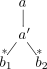
\includegraphics[width=1.6cm]{../newman_2}}
          \hspace{4em}
          \subfloat[\label{fig:newman_b}]{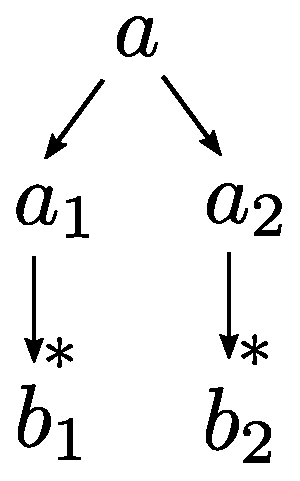
\includegraphics[width=1.5cm]{../newman_1}}
          \hspace{4em}
          \subfloat[\label{fig:newman_c}]{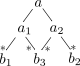
\includegraphics[width=2.7cm]{../newman_3}}\hfill
          \caption{Warianty konstruowania redukcji.} 
        \end{figure}
      \end{minipage}
    \end{center}
  \end{enumerate}
  Stosując powyższe rozumowanie do \(a'\) otrzymujemy kolejny element niejednoznaczny. a zatem możemy skontruować nieskończony ciąg redukcji, wbrew zalożeniu, że relacja \(\to\) jest SN. Zatem \(A\) nie zawiera elementów niejednoznacznych. \qed
\end{dowod}
